\documentclass[paper=a4, fontsize=11pt,twoside]{scrartcl} 

\usepackage[a4paper,pdftex]{geometry}
\setlength{\oddsidemargin}{5mm}
\setlength{\evensidemargin}{5mm}
\setlength{\parindent}{0pt}

\usepackage[english]{babel}
\usepackage[protrusion=true,expansion=true]{microtype}	
\usepackage{amsmath,amsfonts,amsthm,amssymb}
\usepackage{graphicx}
\usepackage{listings}  % Include the listings package
\usepackage{xcolor}
% Configure listings
\lstdefinestyle{mystyle}{
    language=Python,
    basicstyle=\small\ttfamily,
    keywordstyle=\bfseries\color{red!50},
    commentstyle=\color{green!60!purple},
    stringstyle=\color{blue!40},
    numbers=none, 
    numberstyle=\tiny,
    stepnumber=1,
    numbersep=5pt,
    backgroundcolor=\color{white},
    frame=none,
    breaklines=true,
    breakatwhitespace=true,
    tabsize=4,
}

% Define codecell environment
\lstnewenvironment{codecell}[1][]{
    \lstset{style=mystyle, #1}
}{}

% --------------------------------------------------------------------
% Definitions (do not change)
% --------------------------------------------------------------------
\newcommand{\HRule}[1]{\rule{\linewidth}{#1}}

\makeatletter
\def\printtitle{
	{\centering \@title\par}}
\makeatother

\makeatletter
\def\printauthor{
	{\centering \large \@author}}
\makeatother

% --------------------------------------------------------------------
% Metadata
% --------------------------------------------------------------------
\title{
    \normalsize \textsc{Future Computing Technologies Lab: Creative Inquiry} \\ [2.0cm]
	\HRule{0.5pt} \\
	\LARGE \textbf{\uppercase{Semester Report}}
	\HRule{2pt} \\ [0.5cm]
	\normalsize December 6, 2023
}

\author{
	Michael Joseph Ellis\\	
	Clemson University\\	
	Department of Electrical and Computer Engineering\\
	School Email: \texttt{mje2@clemson.edu} \\
}


% --------------------------------------------------------------------
% Main Document
% --------------------------------------------------------------------
\begin{document}

\thispagestyle{empty}

\printtitle
\vfill
\printauthor
\newpage

\setcounter{page}{1}

\section{Introduction}
% In this section you will describe the project that you chose. What data did you work with? What task(s) did you try to perform with the data (visualization, classification, clustering, etc.)? What motivated you to choose these things?

For this project, I centered my subject around Flower Recognition using Convolutional Neural Networks (CNNs). The data set comprises a collection of different flower images organized into different categories. These images were organized within a directory structure, where each category of flowers has its own dedicated sub-directory. Through a systematic exploration of data loading, preprocessing, and visualization, the project emphasizes the importance of having a well-organized dataset in machine learning.\\ 

Throughout this project, I unfold through multiple essential phases in basic machine learning. Quality data checks, class distribution balancing, model evaluation, and a comprehensive understanding of both the dataset and the model's performance are all included. \\

\subsection{Data Used}

For the data, I had to grab it from this website: \\
\texttt{https://www.kaggle.com/datasets/alxmamaev/flowers-recognition}. \\

This data set comprises of images featuring flowers from five different distinct categories. \\ 
Here are the categories -

\begin{itemize}
    \item Dandelions
    \item Daisy
    \item Sunflower
    \item Tulip
    \item Rose
\end{itemize} 

This data set contained a small amount of images, 4242 images to be precise, for my project but it was good enough as a starting point since this is only my first out of many.  

\subsection{Tasks Performed}

The tasks performed during this project were quite numerous.\\ 
So lets go through them. 
\begin{itemize}
    \item \textbf{Data Loading and Preprocessing:} The code loads and preprocesses the image data. Images are then resized, and the pixel values are normalized. 
    \item \textbf{Data Visualization:} Random Samples from the dataset are visualized to get an understanding of the images. Along with multiple visual data tables throughout the project.  
    \item \textbf{Data Quality Checks:} There's a function to check for potential noise in images. 
    \item \textbf{Data Balancing:} The class distribution is balanced by undersampling the majority classes. 
    \item \textbf{Data Splitting:} The balanced dataset is split into training and testing sets.
    \item \textbf{Model Building:} A CNN model is constructed using Tensorflow and Keras. 
    \item \textbf{Model Training and Evaluation:} The model is trained and evaluated on the test set. Training/validation accuracy is plotted. 
    \item \textbf{Model Predictions:} Predictions are made on the test set, and a sample of test images with true and predicted labels is displayed. 
    \item \textbf{Performance Metrics:} F1 score is calculated as a performance metric. 
\end{itemize}

\subsection{Motive}

Handling class imbalance was important, as the project addresses the issue of class imbalance by undersampling, which is crucial for training a more robust and unbiased model. Using appropriate deep learning techniques learned from the Creative inquiry was just as important as well. Utilizing CNN's (Convolutional Neural Networks) are well-suited for image-related tasks, and in this case, they are used for recognizing patterns and features in flower images. Visualization of data and model performance was also essential for understanding how well the model is learning and generalizing from the data. The overall motive behind this project was to build a robust flower recognition model as well as ensuring good data quality.

\section{Materials and Methods}

% In this section you will describe the steps you took in your project. You can be as detailed as you like, including not only what your code does but also how you prepared your data, how you collected results, etc. Someone reading this section should be able to reproduce what you did on a conceptual level. You do not need to include code, but if you do, please include it as an appendix rather than in the text.

Firstly, when starting this project, I had to import a couple of packages and libraries to get going. Initially there was a problem with these imported packages and libraries that was solved later on by switching from Jupyter Notebooks to Google Collab (more on that in the experience section). For this project to work in Google Collab, I had to allow google to access my drive to authorize permission and unzip my downloaded zip file containing all of my data. (See appendix A) \\

Secondly, we had to categorize all the flowers we wanted to classify and state the data directory of the imported data that was within Google Drive. Loading and iterating the data was the next step in the process. Doing this step, I made a list that would store processed image data along with their corresponding class indices. I iterated through each category and constructed a path to the directory containing images for the current category. After doing so, I would assign a unique class index to whatever is the current category in the list to provide a unique numerical identifier for each class. Afterwards I would iterate over each file in the specified category directory. The code then checks if the file has a '.jpg' extention to ensure that it is an image file, and then reads the image using OpenCV ('cv2' library) and loads it as a color image. The images are resized to a fixed size of 150x150 pixels and they are added to a list containing the processed images and their corresponding class index. After this loop is done, the 'features' list will contain pairs of processed images and their corresponding class indices, ready to be used for further processing or training machine learning models. (See appendix B) \\

For this part, we went through all the preprocessing and visualization of the data and distributions. My first step was to initialize two empty lists named 'x' and 'y', and make a loop that would iterate though each element in the previously stated 'features' list, where each element in that list is a pair. The first element of the list is an image array and the second being the class label that was given earlier. For each iteration we append the image array to the 'x' list, and similarly with the 'y' list, we would append all the class labels corresponding to the images. I then had to perform two tasks, converting the lists into NumPy arrays and normalizing the image data by dividing each pixel value by 255.0. For the conversion, we did this for a number of reasons; maintaining memory efficiency, applying efficient numerical operations with NumPy's highly efficient array object, as well as compatibility with other libraries such as Scikit-learn, and Tensorflow to name only the few included in this project. As for the normalizing image data, this is a common preprocessing step in machine learning and deep learning, as it helps to bring all features to a similar scale. For our case of image data, the pixel values are typically in the range of [0, 255], and dividing by 255.0 scales them to a range of [0, 1]. This is done only to ensure that the neural network converges faster during training. Starting for visualization, we created a 2x5 grid of subplots, where 'fig' is the entire figure, and 'ax' is a 2D array of subplots. This means we will have two rows and five columns of subplots. I then set the size of the entire figure to 30 units in width and 15 units in height. The nested for loop iterates over each subplot in the 2x5 grid, and for each subplot, it randomly selects an index from the data set and displays the image corresponding to that index. The subplot's title is set to the corresponding flower category as well. I then visualize the distribution of class labels in the dataset using the 'Seaborn' library. In the next snippet of code, I then visualize the distribution of class labels in the dataset on a countplot using the 'Seaborn' library.  (See Appendix C) \\

Starting up the more interesting stuff, I start to balance my data. This large block of code (See Appendix D), is for balancing the class distribution by undersampling the classes with the majority of data randomly to match the count of the classes with the minority of data. Balancing a dataset can be particularly important when dealing with imbalanced classes in machine learning tasks because it is commonly done to prevent models from being biased towards the classes with the majority of data during training. The code counts the number of samples for each class in the original dataset 'y', and then continues to find the class with the least samples of data, I identify this as the 'min\textunderscore class'. I then perform some random undersampling by initializing empty lists, 'X\textunderscore balanced' and 'y\textunderscore balanced' to store balanced datasets. The code iterates over each class in the original dataset and for each majority class, excluding the minority class , it randomly undersamples the majority class 'X\textunderscore majority' using the 'resample' function. Then the number of samples is set to 'min\textunderscore count' to match the count of the minority class. The sampled data is then added to 'X\textunderscore balanced' and the corresponding labels to 'y\textunderscore balanced'. I also ensure that one sample from the minority class is included in the balanced dataset without undersampling. The code then vertically stacks 'X\textunderscore balanced' to create a NumPy array along with converting 'y\textunderscore balanced' into a NumPy array. Class distribution is then checked after undersampling. The code checks class distrbution in the balanced dataset by using the 'Counter' class. It creates class\textunderscore counts\textunderscore list' to store the counts of each class after balancing. After this is all done, I visualize the class distribution in a pie chart after balancing, showing all the different classes with varied colors. In summary, this code snippet is a method for addressing class imbalance by undersampling the majority classes to balance the distribution evenly across the five classes. This again helps the model from being biased towards any of the previously had majority classes during training.  \\

This next part is setting up for the model training. Firstly, we have to split the data into a training and test set. I use 'X\textunderscore balanced.shape' to obtain the shape of the 'X\textunderscore balanced' dataset, which represents the features of the balanced dataset after undersampling. Specifically, it returns a tuple representing the dimensions of the array 'X\textunderscore balanced'. The shape is typically in the form '(number of samples, number of features)'. The code is checking and printing the shape of the 'X\textunderscore balanced' dataset, providing information about the size and structure of the balanced feature data. For instance, when you see an output like '(n, m, ...)': 'n' represents the number of samples or instances in the balanced dataset and 'm' represents the number of features for each sample. Understanding the shape is important for verifying the structure of data and ensuring that it aligns with the expectations of a machine learning model. The next part is responsible for splitting the balanced dataset into training and testing sets. We use the 'train\textunderscore test\textunderscore split' function from Scikit-learn to shuffle and split the dataset into training and testing sets. The first two parameters are 'X\textunderscore balanced' as features and 'y\textunderscore balanced' as labels. The parameter 'test\textunderscore size = 0.2' specifies that 20\% of the data will be used for testing, and the remaining 80\% will be used as training. The parameter 'random\textunderscore state = 42' seeds the random number generator, ensuring that if you run the same code again, you will get the same split, making the process reproducible later. We get four resulting variables that tell us the features for both the training and testing set along with the labels for the training and testing set. This provides information about the size and structure of each set, which is useful for verifying that the split was done correctly and that the data is ready for training and evaluation. For the next snippet, we use the 'to\textunderscore categorical' function from Keras that converts class vectors to binary class matrices. It takes the original labels ('y\textunderscore train' and 'y\textunderscore test') and the number of classes as parameters. The result is that these two parameters are transformed into one-hot encoded matrices, where each row corresponds to a sample, and each column corresponds to a class. The value in each column is 1 if the sample belongs to that class and 0 otherwise. This format is suitable for training neural networks, especially when using categorical cross-entropy as the loss function. (See Appendix E) \\

This is the part where we start defining, compiling, and training the CNN model using the Keras library. The model definition defines a sequential model as a linear stack of layers. The model consists of convolutional layers with max-pooling and dropout for feature extraction, followed by fully connected layers for classification. For the model compilation, we use the 'Adam' optimizer and for our loss we use 'categorical cross-entropy' which is very suitable for multi-class classification and 'accuracy' as the evaluation metric. During our training, we use image augmentation. We do this by using the 'ImageDataGenerator' function for real-time data augmentation. It specifies many transformations such as rotation, width and height shifts, and horizontal flips to create new images out of already existing ones. Finally the 'model.fit' trains the model on the training data, and the 'validation\textunderscore data = (X\textunderscore test, y\textunderscore test)' uses the validation set during training to monitor model performance. The amount of epochs I used for this was 30 and used a batch size of 32 which is the amount of samples used in each iteration. The next code snippet evaluates the model on the test set. This block uses the 'evaluate' method of the trained model to access its performance on the test set. It takes the test features and corresponding labels as input and returns the loss and accuracy on the test set. These values are then assigned to the variables 'test\textunderscore loss' and 'test\textunderscore acc'. The code then prints out the accuracy to the console. Finally we give a plot for visualization of the training and validation loss of the model. The line plots the training accuracy values stored in the 'history' object from the previous cell and it uses the 'val\textunderscore accuracy' key from the 'history.history' dictionary. In the visualization there is a epoch label on the x-axis and a accuracy label on the y-axis. Overall this visualization was to show how the training and validation accuracy change over epochs to help understand the training process and identify potential overfitting or underfitting issues. (See Appendix F) \\ 

Another part of the project I thought was interesting was the visualization of the images being processed during training. These two last blocks (See Appendix G) are responsible for making predictions on the test set using the trained model and then displaying a random sample of test images along with their true and predicted labels and print the accuracy of the test. I start by using the trained model to make predictions on the test set, resulting in predicted probabilities for each class. The code then extracts the class labels with the highest predicted probability for each image, using 'np.argmax' along with the specified axis to get the indices of the maximum values along the second axis. Similarly, I extract again but this time I do it for the true class labels from the one-hot encoded representation of the true labels in the test set ('y\textunderscore test'). I then define the function 'display\textunderscore images\textunderscore with\textunderscore labels' to visualize a grid of images along with their true and predicted labels. The code randomly selects 25 indices from the test set without replacement, and extracts the images corresponding to the randomly selected indices. It also extracts the true labels corresponding to the randomly selected indices and its predicted labels as well. The function is then called to display the grid of images with their true and predicted labels on a plot. This all helps visualize how well the model performs on a random sample of test images by comparing the true and predicted labels. Finally, we calculate the F1 score, which is a commonly used metric for evaluating the performance of classification models. The F1 score is the harmonic mean of precision and recall. It provides a balance between precision and recall, and is particularly useful when there is an uneven class distribution. A higher F1 score indicates better model performance, considering both false positives and false negatives. The 'micro' average treats all classes equally when computing the F1 score. 

\section{Results}

% In this section you will put any relevant results that you have obtained during the semester. You should focus on results that show the dataset you used as well as the tasks that you were able to accomplish with it. Be sure to explain all tables and figures that you provide. For example, if you have a confusion matrix for a classifier which shows especially low accuracy in a particular class, try to offer an explanation for why the classifier performed poorly with that class. Try to present your results in tables and figures rather than in a sentence so that they are clearly distinguishable.

Regarding the results, I will go over the visualizations and data for the final accuracy.  

\subsection{Class Distribution and Balancing}
As previously stated before, after our preprocessing of the data, we find out the true class distribution of our data. This is a small table of the given visualization from the code. 

\begin{table}[h]
    \centering
    \begin{tabular}{|c|c|}
        \hline
        \textbf{Classes} & \textbf{Count} \\
        \hline
        Dandelion & \textasciitilde 1200 \\
        Daisy & \textasciitilde 790 \\
        Sunflower & \textasciitilde 770 \\
        Tulip & \textasciitilde 980 \\
        Rose & \textasciitilde 800 \\
        \hline
    \end{tabular}
    \caption{Table of Class Distribution}
    \label{tab:xy_values}
\end{table}

After this, we balance our skewed data to prevent bias in our model. This is the new table for our balanced data. 

\begin{table}[h]
    \centering
    \begin{tabular}{|c|c|}
        \hline
        \textbf{Classes} & \textbf{Count} \\
        \hline
        Dandelion & \textasciitilde 770 \\
        Daisy & \textasciitilde 770 \\
        Sunflower & \textasciitilde 770 \\
        Tulip & \textasciitilde 770 \\
        Rose & \textasciitilde 770 \\
        \hline
    \end{tabular}
    \caption{Table of Balanced Class Distribution}
    \label{tab:xy_values}
\end{table}

\subsection{Model Training Accuracy}
For our model training accuracy, display all our loss, accuracy, val\textunderscore loss, and val\textunderscore accuracy, after each of our epochs are done with their steps and how long it took to execute (92 steps each for 30 epochs). At the end I came to a conclusion of 80.76\% test accuracy. Initially I could have stopped the epochs at around 27 since it had the highest validation accuracy out of all the epochs. 

\begin{table}[h]
    \centering
    \begin{tabular}{|c|c|c|c|c|}
        \hline
        \textbf{Epochs} & \textbf{Loss} & \textbf{Accuracy} & \textbf{Val\textunderscore Loss} & \textbf{Val\textunderscore Accuracy}\\
        \hline
        Epoch 1/30 & 1.5899 & 0.3417 & 1.2143 & 0.5416 \\
        Epoch ... & ... & ... & ... & ... \\
        Epoch ... & ... & ... & ... & ... \\
        Epoch ... & ... & ... & ... & ... \\
        Epoch 27/30 & 0.0110 & 0.9959 & 1.3333 & 0.8158 \\
        Epoch 28/30 & 0.0073 & 0.9980 & 1.3868 & 0.7967 \\
        Epoch 29/30 & 0.0073 & 0.9983 & 1.3590 & 0.8158 \\
        Epoch 30/30 & 0.0079 & 0.9983 & 1.3801 & 0.8076 \\
        \hline
    \end{tabular}
    \caption{Table of Model Evaluations}
    \label{tab:xy_values}
\end{table}

On a short note, inside of all of those epochs I visualized a prediction of what the model might be doing. 

\begin{table}[h]
    \centering
    \begin{tabular}{|c|c|c|}
        \hline
        \textbf{True} & \textbf{Predicted} & \textbf{Correct?} \\
        \hline
        Tulip & Tulip & Yes \\
        Dandelion & Sunflower & No \\
        Sunflower ... & ... & ... \\
        Rose ... & ... & ... \\
        Daisy & Daisy & Yes \\
        \hline
    \end{tabular}
    \caption{Table of Predicted Model Evaluations from Epoch \#30}
    \label{tab:xy_values}
\end{table}


\section{Experience}

% \textit{This section is especially important.} In this section you will describe your overall experience in the CI. What did you enjoy? How do you think the CI could be improved (please don't hesitate to speak freely)? What new skills did you learn? What challenges did you face, and if applicable, how did you overcome them? What topics were you exposed to that are otherwise inaccessible to undergraduate students? Is there anything that you would like to pursue in the future as a result of your participation in the CI? If the CI has had any impact on your understanding of graduate research or interest in pursuing a graduate degree, feel free to include that here as well.

Participating in the CI has been an incredibly enjoyable and interesting experience for me. I found the entire journey to be sufficient intellectually and weirdly stimulating, providing me with opportunities to delve into intriguing topics and engage in collaborative research that is often beyond the reach of undergraduate coursework. One of the aspects I enjoyed the most was the exposure to advanced topics that are not typically covered in traditional undergraduate settings. The CI opened doors to areas like supervised and unsupervised learning, dense layers, and convolutional layers which have deepened my understanding and sparked a genuine interest in their complexity. During classes, with the help of Max and Adam I was able to understand a lot of the topics we went over in depth due to the amount of clarity they provided. Throughout the CI, I encountered challenges that was mainly from Jupyter Notebook being a bit outdated and uncomfortable to use in some areas. Although every other obstacle served as a valued learning opportunity, Jupyter Notebook was the one thing I couldn't figure out until realizing how outdated it was funnily enough. Though, overcoming challenges during my project has undoubtedly enhanced my problem-solving skills and resilience. The collaborative nature of the program given by Max and Adam fostered a supportive environment for me and other undergraduates where we could all seek guidance. Their exposure has been instrumental in shaping my aspirations for the future, and I'm now considering Machine Learning and AI as a potential path for future exploration. This CI has had a great impact on my perception of graduate research, sparking a genuine interest in pursuing advanced studies. The immersive and hands-on nature of the program has exposed me to the some small aspects of the research process, which has made me more confident in my ability to contribute meaningfully to academic endeavors in the future. Reflecting on my overall experience in the CI, I believe that having more topics to go over would be great to have. Nevertheless, I am immensely grateful for the opportunity to have been part of the class, and I am excited about the potential avenues it has opened for me in the future. 


\section{Conclusions and Future Work}

% In this section you can make conclusions about the results that you obtained during the semester. What are the potential "next steps" for your project, should you choose to continue it? Additionally, you can include any ideas for other projects that you would like to work on, or even general suggestions for projects that you think would fit well in the CI.

I think overall I am happy with my results and where I stood with my data and how I managed to use it. Looking into the future for my "next steps" in my project if I chose to continue it, I think I'd want to look into how I can make my accuracy better and look into how else I could make my overall project as a whole better. I think learning more about the topics 'reinforced learning' and 'natural language processing' would peak my interest more in the CI class and would really like to see how that's implemented for the class if not, then maybe other really interesting topics. \\

% \section{Appendices}
\newpage
\LARGE \chapter*{Appendices} \\ % Use \chapter* to create an unnumbered chapter for appendices

\begin{figure}[h]
    \centering
    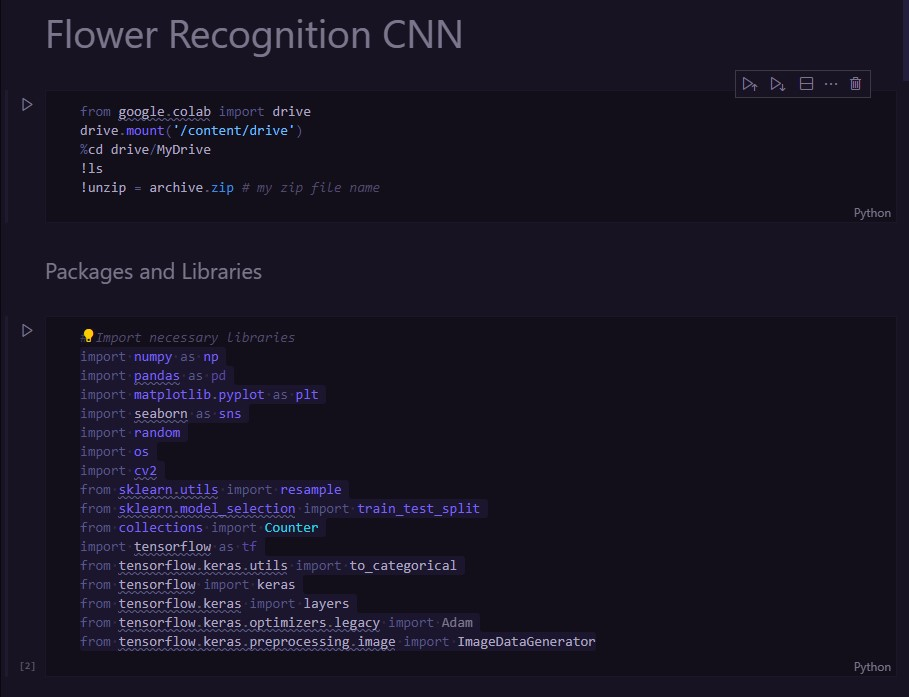
\includegraphics[width=0.8\linewidth]{Cells 1 and 2.jpg}
    \caption{Appendix A}
    \label{fig:appendix_image_a}
\end{figure}

\begin{figure}[h]
    \centering
    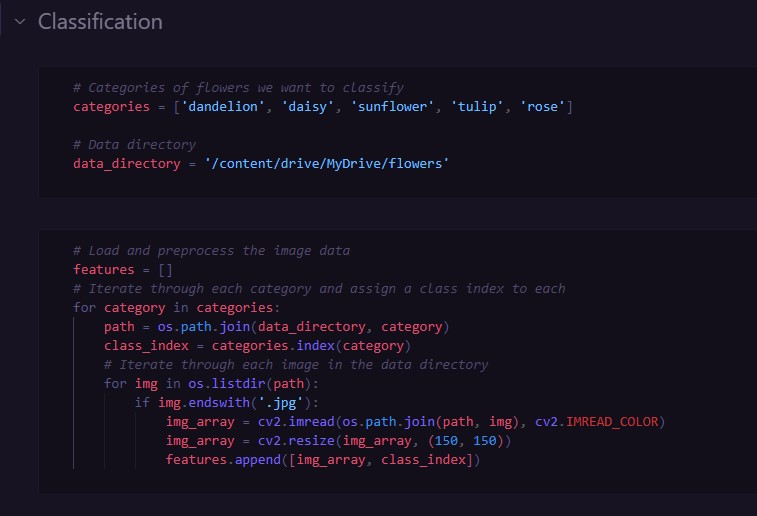
\includegraphics[width=0.8\linewidth]{Cells 3 and 4.jpg}
    \caption{Appendix B}
    \label{fig:appendix_image}
\end{figure}

\begin{figure}[h]
    \centering
    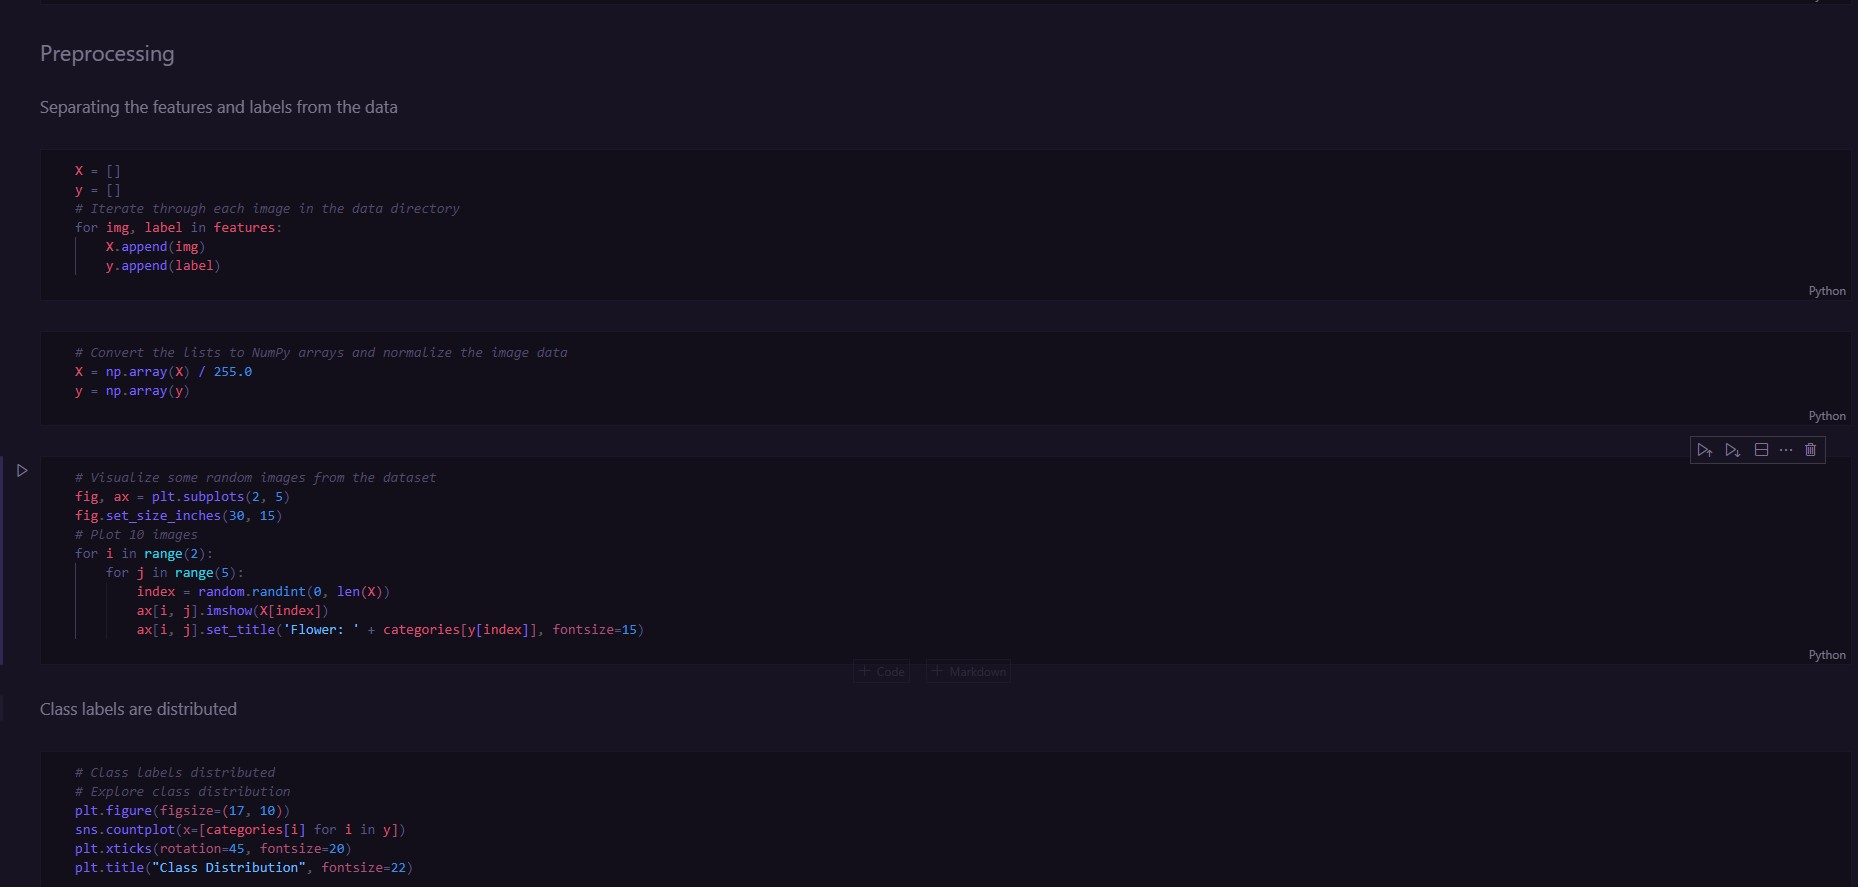
\includegraphics[width=0.8\linewidth]{Cells image3.jpg}
    \caption{Appendix C}
    \label{fig:appendix_image}
\end{figure}


\begin{figure}[h]
    \centering
    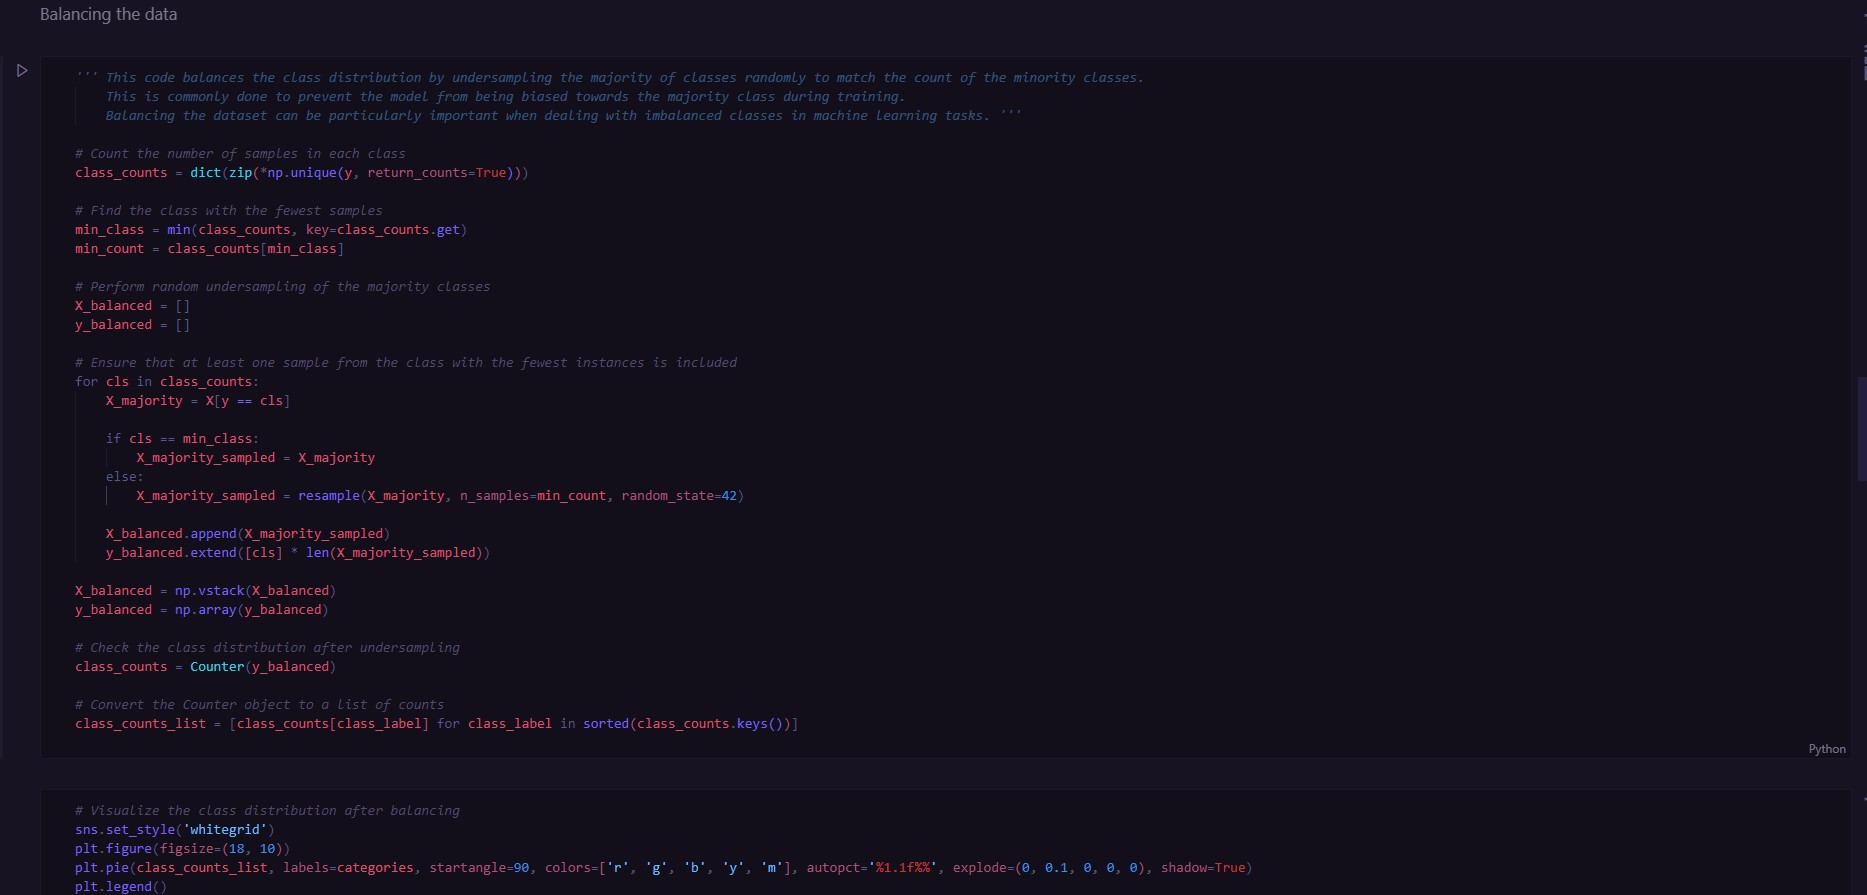
\includegraphics[width=0.8\linewidth]{cells image 4.jpg}
    \caption{Appendix D}
    \label{fig:appendix_image}
\end{figure}


\begin{figure}[h]
    \centering
    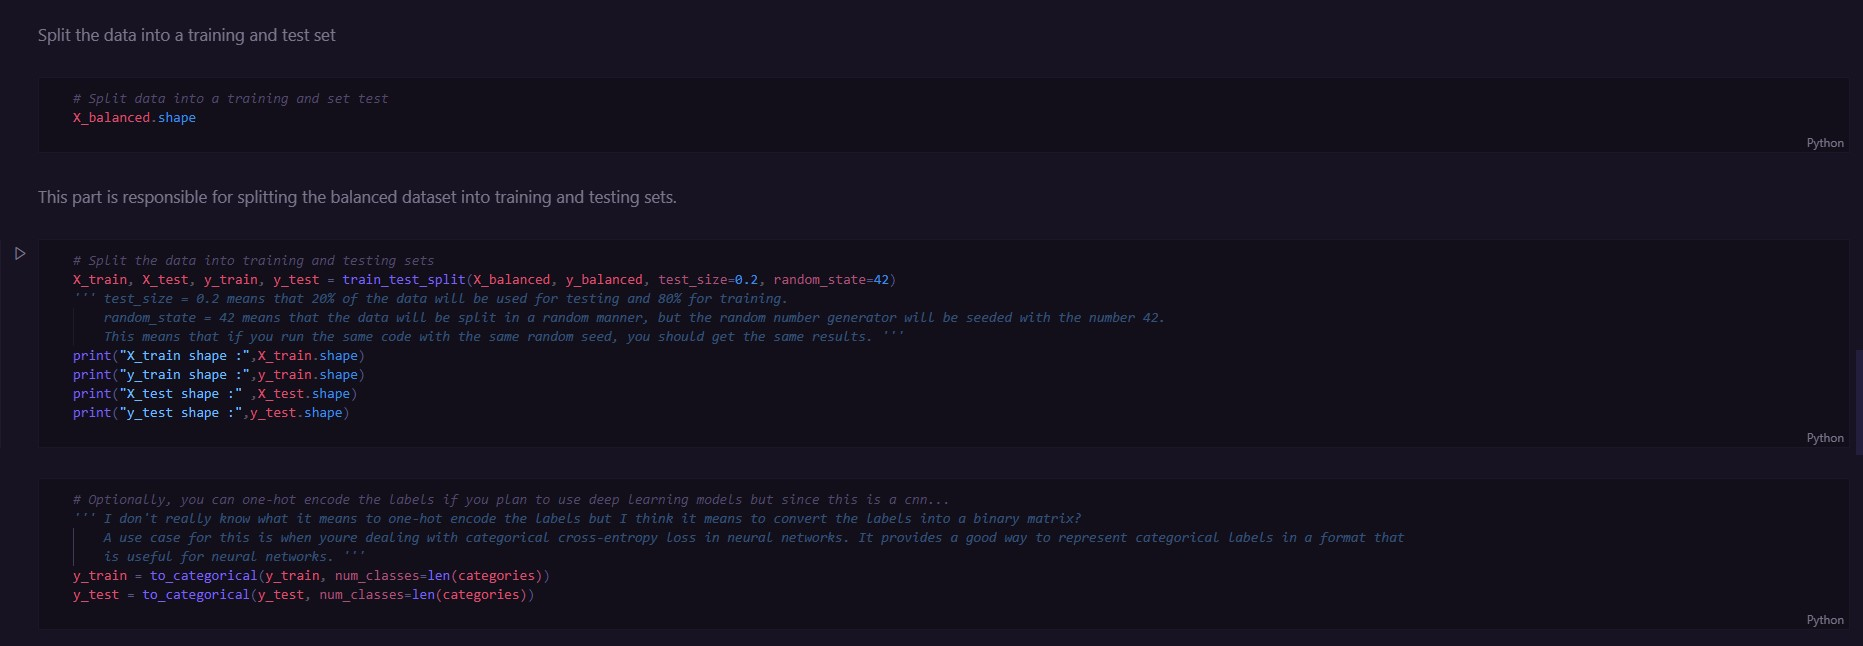
\includegraphics[width=0.8\linewidth]{cells image 5.jpg}
    \caption{Appendix E}
    \label{fig:appendix_image}
\end{figure}


\begin{figure}[h]
    \centering
    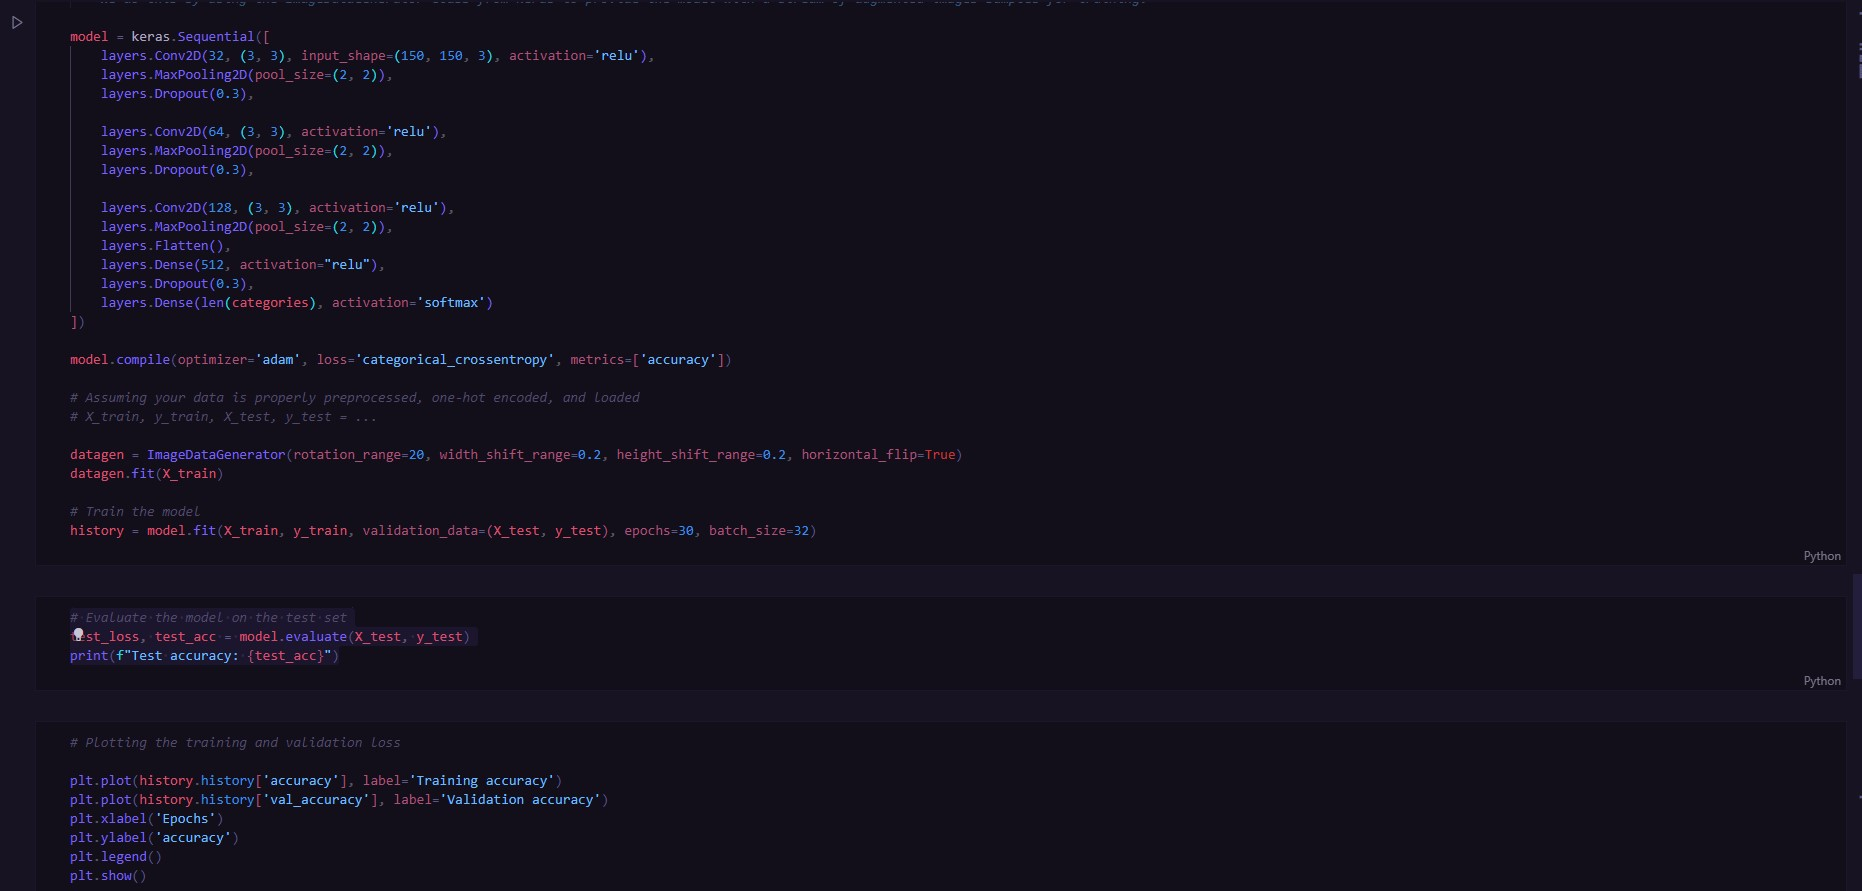
\includegraphics[width=0.8\linewidth]{cells image 6.jpg}
    \caption{Appendix F}
    \label{fig:appendix_image}
\end{figure}


\begin{figure}[h]
    \centering
    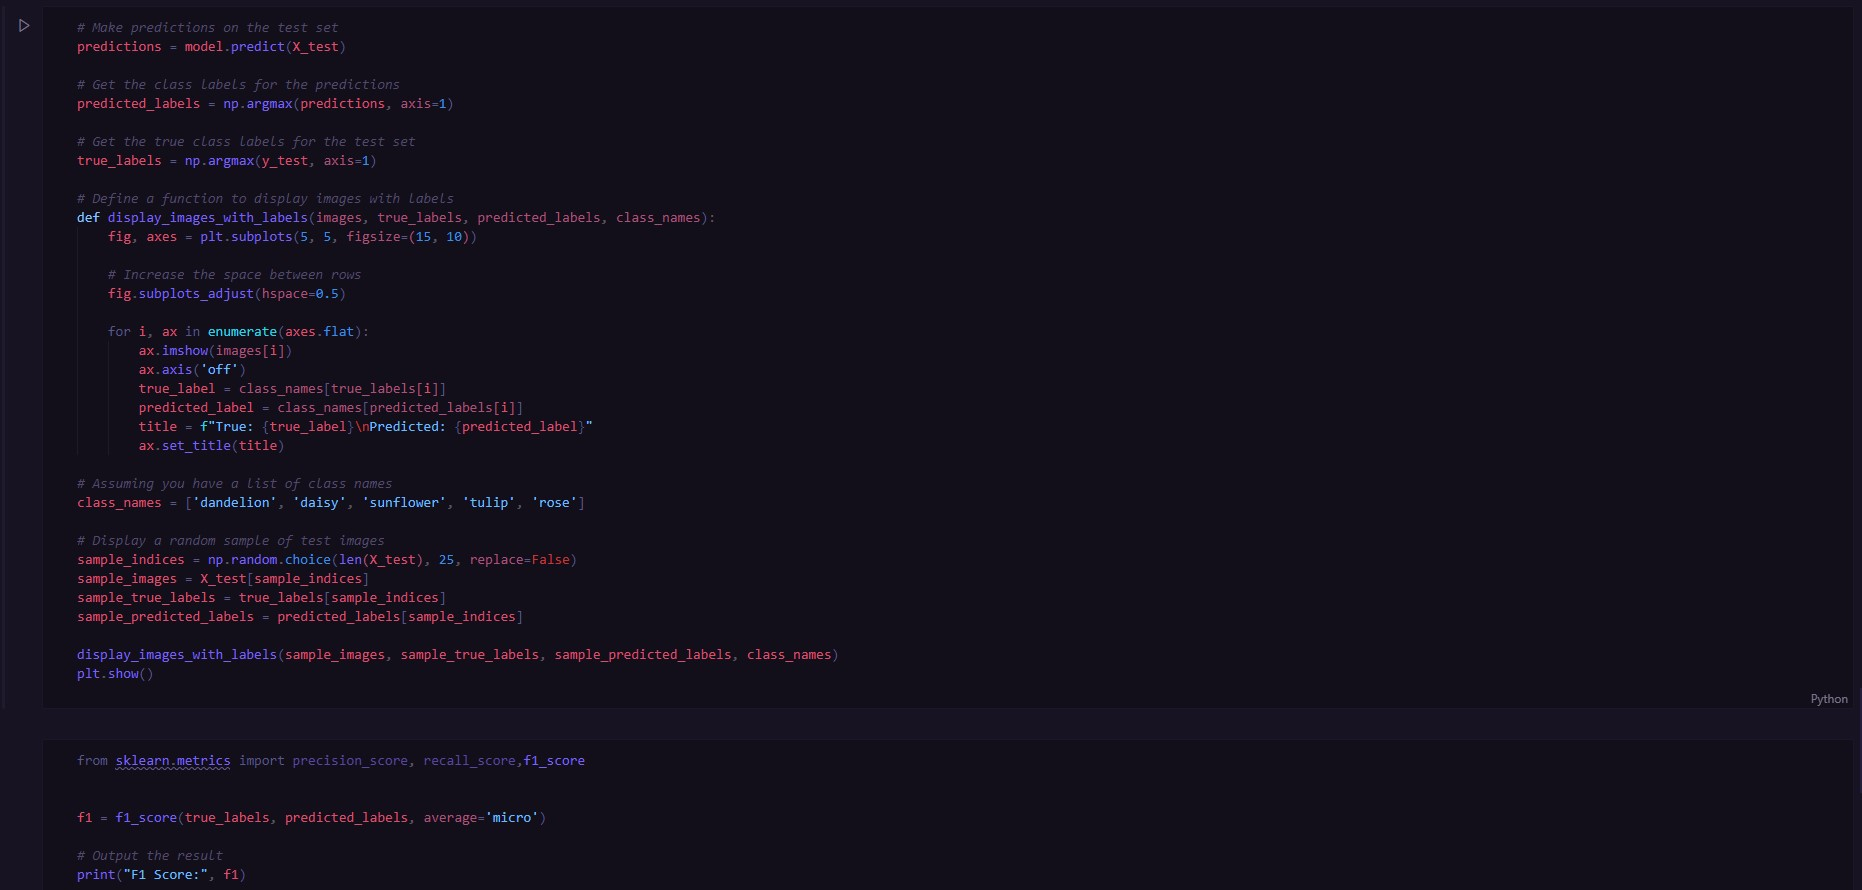
\includegraphics[width=0.8\linewidth]{cells image 7.jpg}
    \caption{Appendix G}
    \label{fig:appendix_image}
\end{figure}


\end{document}
